\documentclass[10pt,twocolumn]{article}
\usepackage[margin=0.66in,columnsep=0.28in]{geometry}
\usepackage{times}
\usepackage{graphicx}
\usepackage{booktabs}
\usepackage{amsmath}
\usepackage{xcolor}
\usepackage{hyperref}
\usepackage{caption}
\usepackage{titlesec}
\usepackage{enumitem}
\setlist{nosep,leftmargin=1.1em}
\titlespacing*{\section}{0pt}{1.0ex plus 0.3ex minus 0.2ex}{0.5ex}
\titlespacing*{\subsection}{0pt}{0.7ex plus 0.2ex}{0.3ex}
\hypersetup{colorlinks=true,linkcolor=black,citecolor=black,urlcolor=blue!50!black}
\setlength{\parindent}{0pt}
\setlength{\parskip}{0.16em}

\title{\vspace{-2.6em}\textbf{SPACE: Style-Preserving Attribute-Constrained Erasure for\\ Artist-Style Unlearning in Text-to-Image Diffusion Models}\vspace{-0.8em}}
\author{\normalsize Team ngmi --- Vedang Pandey \\ \small Gen$\mu$ 2.0 Challenge --- Track 3: Visual Concept Unlearning \\ \small \href{https://github.com/Vedang-P/genmu2026-space-submission}{github.com/Vedang-P/genmu2026-space-submission}}
\date{}

\begin{document}
\twocolumn[
\maketitle
\vspace{-2.4em}
\centerline{\parbox{0.94\textwidth}{\small\noindent\textbf{Abstract.} We present SPACE (Style-Preserving Attribute-Constrained Erasure), a preservation-first method for erasing artist styles from Stable Diffusion v1.4. Rather than treating erasure strength and content/quality preservation as a single objective to be traded off, SPACE edits a frozen base model with saliency-selected LoRA adapters trained against a dual-anchor teacher that simultaneously anchors toward neutral, content-preserving output and explicitly subtracts an estimated target-style residual. We validate SPACE on two independent target concepts --- Vincent van Gogh (submission target) and Thomas Kinkade (independent replication) --- using a standardized protocol of 500 matched target-prompt pairs and a full 30{,}000-image FID evaluation against the official MS-COCO 2014 reference set. SPACE reaches FID within 0.07--0.08 of the unedited base model (14.57 vs.\ 14.50 for Van Gogh; 14.58 vs.\ 14.50 for Thomas Kinkade) while measurably suppressing target style (style-score drop 0.045--0.064, target-style hit-rate 32--48\%), showing that broad generative utility and targeted style suppression are jointly achievable rather than mutually exclusive.}}
\vspace{0.8em}
]

\section{Introduction}
Text-to-image diffusion models memorize and reproduce recognizable artist styles, raising copyright and consent concerns and motivating \emph{concept erasure} (machine unlearning) methods. Prior approaches make different trade-offs: ESD~\cite{esd} moves target-concept predictions away from the original via gradient descent, but erasure strength can trade hard against content and quality; UCE~\cite{uce} solves a closed-form edit over erased/preserved concepts, but is not trajectory-aware and treats each prompt as a single point rather than a factorized content/style pair; Concept Ablation~\cite{conceptablation} maps a target concept toward a generic anchor, which looks pleasing but can under-erase and damage nearby concepts.

SPACE's premise is that erasure and preservation should be \emph{jointly engineered}, not opposing forces in one loss term. It factorizes each target prompt into content, target-style, neutral-art, and generic-image views; builds a teacher that anchors toward neutral content \emph{and} explicitly subtracts the estimated style residual; edits only a saliency-selected, low-rank subset of cross-attention projections; supervises across multiple denoising trajectory bands; and replays both general prompts and CLIP-mined \emph{vulnerable} nearby styles during training to bound collateral damage.

\section{Method}
\textbf{Prompt views.} For a target prompt $p_t$ (e.g.\ \emph{``Bedroom in Arles by Vincent van Gogh''}), SPACE constructs a content-only prompt $p_c$ (artist phrase stripped), a neutral art anchor $p_a$ (\emph{``a high quality painting of \{content\}''}), and a generic image anchor $p_g$ (\emph{``a high quality image of \{content\}''}), plus robust paraphrase variants of $p_t$ (\emph{``in the style of'', ``inspired by'', ``as painted by''}) so the edit is not tied to one literal surface form.

\textbf{Teacher construction.} Let $\epsilon_\theta$ be the frozen base U-Net and $x_t$ a noisy latent at timestep $t$. The SPACE teacher is
\begin{align}
n &= (1-\alpha)\,\epsilon_\theta(x_t,\tau(p_c)) + \alpha\,\epsilon_\theta(x_t,\tau(p_a)) \notag\\
d &= \epsilon_\theta(x_t,\tau(p_t)) - \epsilon_\theta(x_t,\tau(p_c)) \notag\\
\text{teacher} &= n - \beta\, d, \label{eq:teacher}
\end{align}
with $\alpha{=}0.30$ and $\beta{=}1.0$ by default. Eq.~\ref{eq:teacher} both anchors the target prompt toward a neutral, content-preserving prediction \emph{and} explicitly pushes away from the target-style direction $d$, rather than only imitating a generic replacement distribution.

\textbf{Student.} The base U-Net is frozen; SPACE trains only LoRA adapters (rank 8) inserted into a saliency-selected subset of cross-attention linear projections. Saliency is measured by probe-gradient norm on a small target/band subset; the top quartile of candidates is edited, so the edited set is data-dependent, not a fixed layer list. The ``teacher'' is the same U-Net with adapters disabled --- no separate frozen expert network is needed.

\textbf{Loss.} Training supervises three trajectory bands ($t\!\in\!\{0.2,0.5,0.8\}$) with
\begin{multline}
\mathcal{L} = \mathcal{L}_{\text{erase}} + \lambda_s\mathcal{L}_{\text{style}} + \lambda_c\mathcal{L}_{\text{content}} + \lambda_i\mathcal{L}_{\text{image}} \\
+ \lambda_p\mathcal{L}_{\text{preserve}} + \lambda_v\mathcal{L}_{\text{vuln}} + \lambda_r\mathcal{L}_{\text{lora}}, \notag
\end{multline}
where $\mathcal{L}_{\text{erase}}$ matches the student's target-prompt prediction to the teacher; $\mathcal{L}_{\text{style}}$ penalizes projected energy onto a rank-4 \emph{style subspace} built by SVD over several target-prompt variants (not a single residual vector); $\mathcal{L}_{\text{content}}$/$\mathcal{L}_{\text{image}}$ anchor $p_c$/$p_g$ to the frozen base model; $\mathcal{L}_{\text{preserve}}$ replays general prompts from a 30k COCO pool on an independently sampled latent; $\mathcal{L}_{\text{vuln}}$ replays CLIP-mined nearby artist styles most at risk of collateral damage; and $\mathcal{L}_{\text{lora}}$ regularizes adapter magnitude. Training uses a two-stage curriculum (300 narrow-supervision steps, then 100 steps with broader prompt-family and style-basis coverage), learning rate $10^{-4}$.

\section{Experimental Setup}
\textbf{Base model.} CompVis Stable Diffusion v1.4, edited in place; no architecture changes.

\textbf{Target concepts.} \emph{Vincent van Gogh} (submission target) and \emph{Thomas Kinkade} (independent second concept, identical protocol), each trained and evaluated separately.

\textbf{Protocol.} 50 target prompts $\times$ 10 samples = 500 matched vanilla/SPACE pairs per concept, plus 30{,}000 SPACE generations over a fixed COCO prompt/seed set, scored by canonical \texttt{torch-fidelity} FID against the official MS-COCO~2014 validation reference --- the same protocol ESD~\cite{esd} reports vanilla SD v1.4 FID (14.50) under.

\textbf{Baselines.} During development, SPACE was benchmarked against ESD-x, UCE, and Concept Ablation on a shared 50-prompt Van Gogh set using official upstream implementations (not reimplementations), all released in the accompanying repository.

\textbf{Metrics.} FID (general utility); CLIP image similarity and DINO similarity (edited-vs-vanilla structural/content agreement); CLIP style score \emph{drop} and \emph{target rate} (fraction of forget-set samples still hitting the target style --- erasure strength); LPIPS (perceptual distance).

\section{Results}
Table~\ref{tab:results} reports both concepts under the identical protocol. FID stays within 0.07--0.08 of the unedited model at 30k-image scale for both concepts, indicating general image quality and prompt-following ability on unrelated content are essentially undamaged. At the same time, target-style hit rate drops to 32.4\% (Van Gogh) and 48.4\% (Thomas Kinkade) with a corresponding CLIP style-score drop, showing real, measurable suppression of the target style rather than a null edit.

\begin{table}[h]
\centering\small
\setlength{\tabcolsep}{3.2pt}
\begin{tabular}{lrr}
\toprule
\textbf{Metric} & \textbf{Van Gogh} & \textbf{T.\ Kinkade} \\
\midrule
FID (30k, canonical) & \textbf{14.57} & \textbf{14.58} \\
\quad vs.\ vanilla SD v1.4~\cite{esd} & 14.50 & 14.50 \\
CLIP image similarity $\uparrow$ & 0.798 & 0.755 \\
DINO similarity $\uparrow$ & 0.622 & 0.471 \\
Style target rate $\downarrow$ & 0.324 & 0.484 \\
Style score drop $\uparrow$ & 0.045 & 0.064 \\
LPIPS (vs.\ vanilla) & 0.569 & 0.578 \\
\bottomrule
\end{tabular}
\caption{SPACE results, 500 matched pairs + 30k-image COCO FID per concept. $\uparrow$/$\downarrow$: higher/lower is better for erasure-preservation trade-off.}
\label{tab:results}
\vspace{-0.5em}
\end{table}

That the same hyperparameters transfer across two stylistically distinct artists (Van Gogh's post-impressionist brushwork vs.\ Kinkade's luminist realism) without per-concept retuning supports that the erasure-preservation trade-off is a property of the method, not an artifact of one target.

\textbf{Qualitative.} Fig.~\ref{fig:qual} shows representative pairs: SPACE consistently removes the signature stylistic cue (Van Gogh's impasto brushwork; Kinkade's diffuse warm-light glow) while retaining scene layout and subject identity. The full 500-pair grids and per-concept metric dashboards are released with the code.

\begin{figure}[h]
\centering
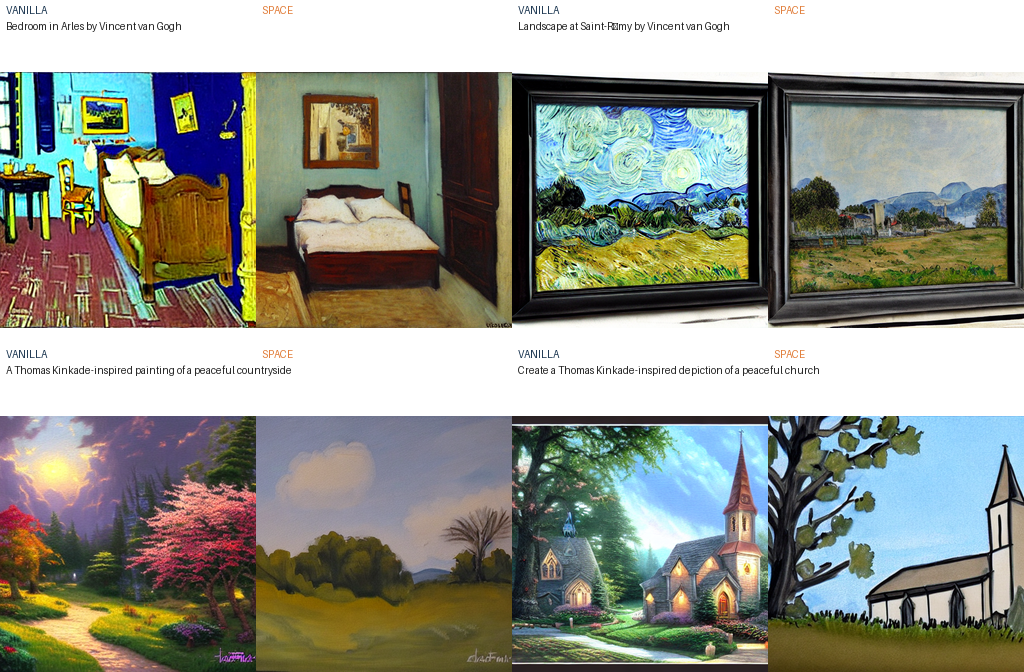
\includegraphics[width=\linewidth]{report_assets/qualitative_figure.png}
\caption{Vanilla SD v1.4 vs.\ SPACE, matched seed/prompt. Top: Van Gogh. Bottom: Thomas Kinkade.}
\label{fig:qual}
\vspace{-0.5em}
\end{figure}

\textbf{Published baseline context.} Under each method's own protocol (not re-run here): UCE reports FID-SD 14.37 erasing one artist vs.\ its SD baseline 14.49~\cite{uce}; ESD's COCO-30k table reports FID 13.68 only for the global nudity-removal variant ESD-u vs.\ SD 14.50, and reports no COCO-30k FID for the style-erasure variant ESD-x we benchmark against~\cite{esd}; Concept Ablation reports FID 16.99 (ablated) vs.\ 16.35 (pretrained) under a 50-step DDPM sampler~\cite{conceptablation}. Differing samplers, guidance, and image counts make these context only, not directly comparable to Table~\ref{tab:results} or each other.

\section{Discussion and Limitations}
A minority of Van Gogh prompts (e.g.\ \emph{``The Reaper''}, \emph{``Cypresses''}) drift toward a recurring dark-robed-figure motif rather than a close content match, so the content anchor does not perfectly constrain every prompt. Style target rate (32--48\%) shows suppression is substantial but not absolute; adversarial or indirect phrasings were not exhaustively probed and are a natural next robustness check. SPACE targets \emph{output-level} style suppression under this harness --- not a formal proof that target-concept information is fully removed from model weights.

\section{Conclusion}
SPACE combines a dual-anchor, style-residual-subtracting teacher with localized LoRA adapters and multi-axis preservation replay to erase artist style while keeping FID within a fraction of a point of the unedited model. Validated identically on two concepts; code, weights, and forget/retain samples are released for reproduction at the repository above.

\begin{thebibliography}{9}
\small
\setlength{\itemsep}{0pt}
\setlength{\parskip}{0pt}
\bibitem{esd} Gandikota, R., Materzynska, J., Fiotto-Kaufman, J., Bau, D. Erasing Concepts from Diffusion Models. \emph{ICCV}, 2023.
\bibitem{uce} Gandikota, R., Orgad, H., Belinkov, Y., Materzynska, J., Bau, D. Unified Concept Editing in Diffusion Models. \emph{WACV}, 2024.
\bibitem{conceptablation} Kumari, N., Zhang, B., Wang, S.-Y., Shechtman, E., Zhang, R., Zhu, J.-Y. Ablating Concepts in Text-to-Image Diffusion Models. \emph{ICCV}, 2023.
\end{thebibliography}

\end{document}
